\section{Laboratory work implementation}

\subsection{Tasks and Points}

\begin{center}
\begin{itemize}
\item \textit{Basic level(nota 5 / 6)}
\begin{itemize}
\item Realizarea un mini site cu 3 pagini statice.
\end{itemize}
\end{itemize}
\end{center}

\subsection{Analiza lucrarii de laborator}

Efectuind aceasta lucrare de laborator am realizat un simplu Web site cu 3 pagini unde fiecare pagina are continutul ei inparte.Acest web site este destinat fanilor unui dintre cele mai populare jocuri din lume CS:GO(Counter Strike Global Offensive).
\\
Prima pagina este un scurt istoric deespre cele mai populare si mai profesional echipe de jucatori in CS:GO , care eu obtinut o mulltime de victorii in campionatele de CS:GO si nu numai pe linga asta  si la jocurile Dota etc.
\\A doua pagina este o pagina destinata noutatilor care apar  despre noi jocuri noi echipe noi campion si a multor altele. \\
A treia pagina este destinata unui portofoliu de skin-uri din joaca CS:GO , sunt prezente o parte din intreaga majoritatea a lor.
\subsection{Imagini}
\textbf{Home}\\
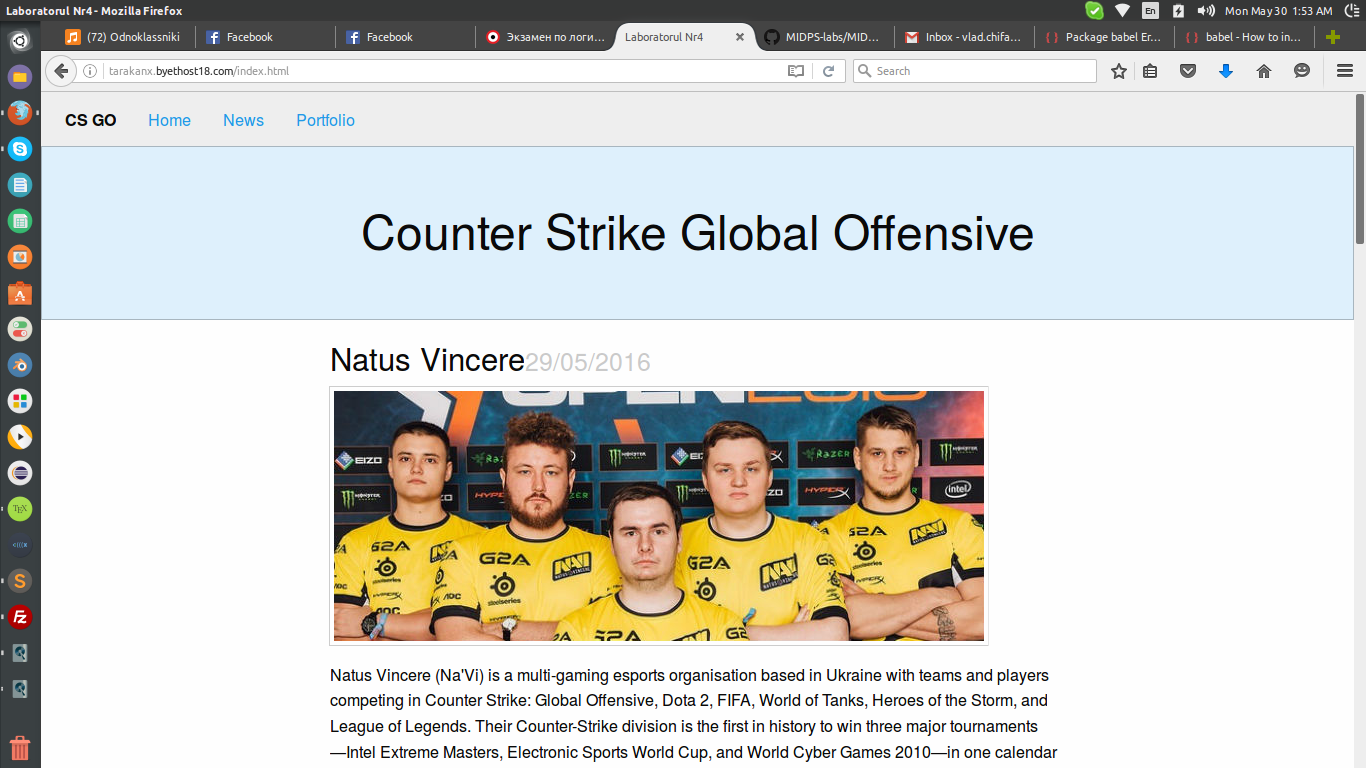
\includegraphics[scale=0.3]{imagini/Home.png} \\
\newpage
\textbf{News}\\
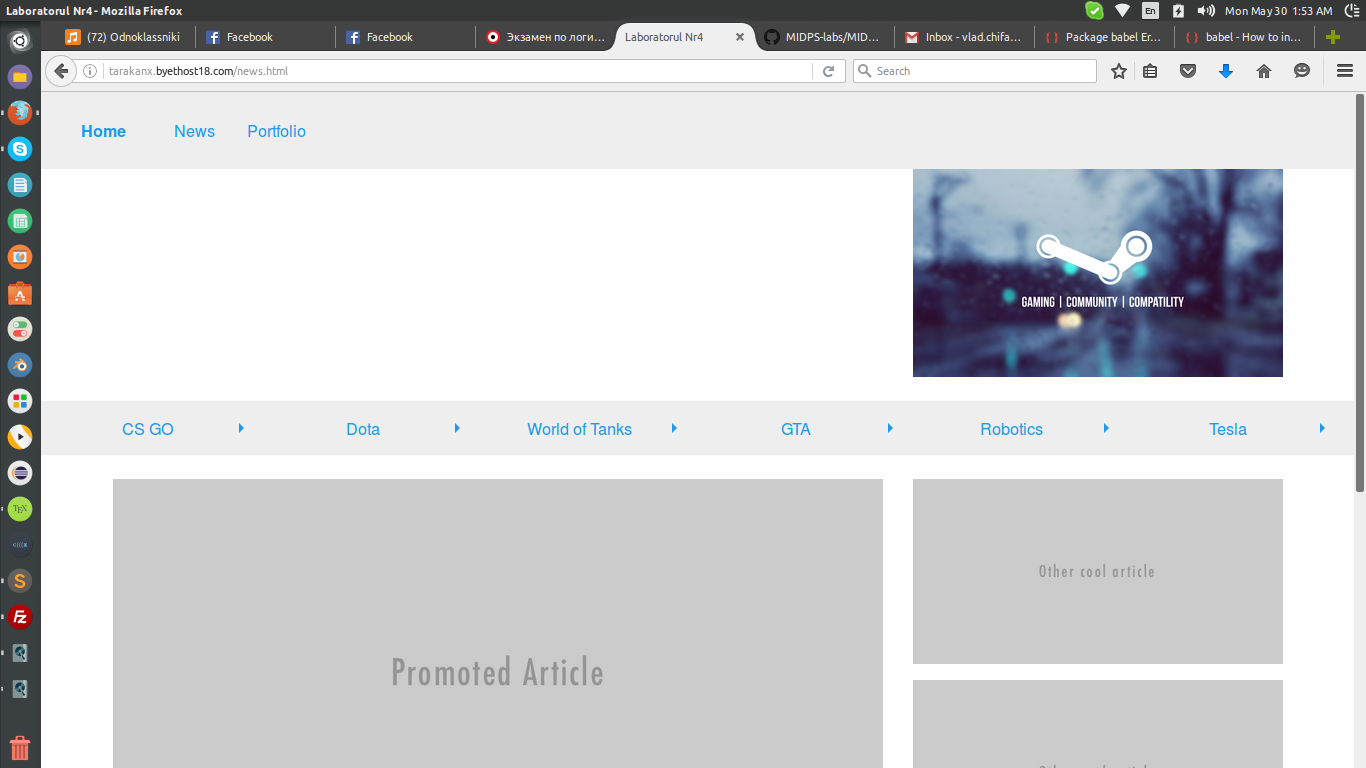
\includegraphics[scale=0.3]{imagini/news.png} \\
\textbf{Portfolio}\\
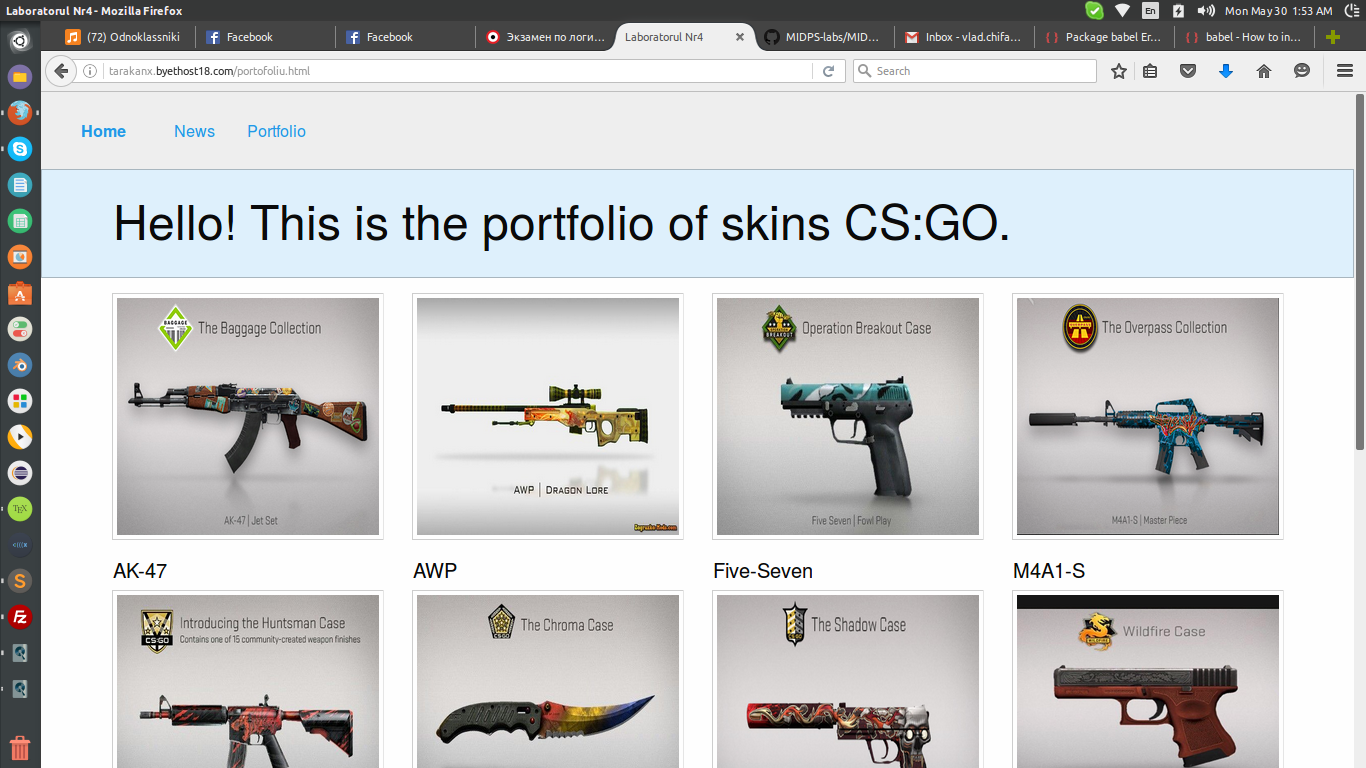
\includegraphics[scale=0.3]{imagini/slide.png} 


\clearpage